\chapter{Background}
\label{Chapter2}
\lhead{Chapter 2. \emph{Background}} % Change X to a consecutive number; this is for the\b\subsection{L\beLocation ve\begin{figure}
\section{\textbf{Dynamic Spectrum Access}}

Dynamic Spectrum Access (DSA) represents a paradigm shift from traditional static spectrum allocation to more flexible and efficient spectrum utilization strategies. Akyildiz et al. \cite{ref3} established the foundational framework for next generation dynamic spectrum access networks, highlighting how DSA enables more efficient spectrum utilization by allowing secondary users to opportunistically access underutilized spectrum bands. The traditional spectrum management approach, where specific frequency bands are permanently allocated to licensed users, often results in significant spectrum underutilization, as many allocated bands remain idle for extended periods.

The DSA paradigm addresses spectrum scarcity issues by implementing intelligent spectrum sharing mechanisms that can adapt to changing spectrum demands and availability \cite{ref2,ref3}. This approach enables unlicensed secondary users to access licensed spectrum bands when primary users are not actively transmitting, thereby maximizing overall spectrum efficiency. The implementation of DSA requires sophisticated sensing, decision-making, and spectrum management capabilities that form the foundation of modern cognitive radio systems \cite{ref25}.

\section{\textbf{Cognitive Radio}}

Cognitive Radio (CR) technology represents an intelligent wireless communication system capable of learning from and adapting to its environment to optimize spectrum utilization. Alias and Ragesh \cite{ref2} provided a comprehensive survey of cognitive radio networks, emphasizing how cognitive radios can dynamically adjust their transmission parameters based on spectrum availability and environmental conditions. The cognitive radio concept was originally proposed to address the inefficient utilization of spectrum resources under traditional static allocation schemes.

A cognitive radio system possesses several key capabilities including spectrum sensing to detect spectrum holes, spectrum decision to select optimal channels, spectrum sharing to coordinate access among multiple users, and spectrum mobility to maintain seamless communication during transitions \cite{ref3,ref25}. These capabilities enable cognitive radios to operate as intelligent agents that can perceive their radio environment, learn from experience, and make autonomous decisions to optimize communication performance while avoiding interference with licensed primary users \cite{ref2}.

The cognitive radio paradigm introduces the concept of primary and secondary users, where primary users have licensed rights to specific spectrum bands, while secondary users can opportunistically access these bands when not in use by primary users. This hierarchical access model requires sophisticated coordination and protection mechanisms to ensure that secondary user activities do not interfere with primary user communications \cite{ref3,ref7}.

\section{\textbf{Spectrum Sensing}}

Spectrum sensing is a fundamental capability of cognitive radio systems that enables the detection of primary user activity and identification of spectrum opportunities. Parvin et al. \cite{ref25} highlighted spectrum sensing as a critical component of cognitive radio network security, as accurate sensing is essential for both efficient spectrum utilization and protection of primary users from harmful interference. The spectrum sensing process involves continuously monitoring the radio frequency environment to determine the presence or absence of primary user signals.

Several spectrum sensing techniques have been developed, including energy detection, matched filter detection, and cyclostationary feature detection \cite{ref1,ref11}. Energy detection is the most commonly used approach due to its simplicity and low computational requirements, but it suffers from performance degradation in low signal-to-noise ratio environments. Cyclostationary feature detection exploits the periodic statistical properties of communication signals and can achieve better performance than energy detection, particularly in noisy environments \cite{ref11}.

The accuracy of spectrum sensing is crucial for cognitive radio operation, as false alarms lead to underutilization of available spectrum, while missed detections can cause harmful interference to primary users \cite{ref1,ref4}. Collaborative spectrum sensing, where multiple cognitive radio nodes share their sensing observations, has been proposed to improve sensing accuracy and reliability \cite{ref8}. However, this collaborative approach introduces new security vulnerabilities, including spectrum sensing data falsification attacks and primary user emulation attacks \cite{ref7,ref14}.

\section{\textbf{Cognitive Radio Networks}}

Cognitive Radio Networks (CRNs) represent the network-level implementation of cognitive radio technology, where multiple cognitive radio nodes coordinate their spectrum access decisions to achieve efficient and harmonious spectrum sharing. Akyildiz et al. \cite{ref3} described CRNs as next-generation wireless networks that can intelligently adapt to changing spectrum conditions and user demands. These networks implement distributed algorithms for spectrum management, interference coordination, and quality of service provisioning.

CRNs can be organized in various architectural configurations, including centralized, distributed, and hybrid approaches \cite{ref2}. In centralized architectures, a central entity collects spectrum sensing information from all network nodes and makes global spectrum allocation decisions. Distributed architectures allow individual nodes to make autonomous spectrum access decisions based on local information and coordination protocols. Hybrid approaches combine elements of both centralized and distributed control to balance efficiency and scalability \cite{ref3}.

The implementation of CRNs introduces several technical challenges, including spectrum sensing accuracy, dynamic spectrum allocation, interference management, and security threats \cite{ref25}. Security concerns are particularly critical, as the open and dynamic nature of CRNs creates opportunities for various attacks, including primary user emulation attacks, spectrum sensing data falsification, and jamming attacks  \cite{ref7,ref16}. These security challenges require the development of robust detection and mitigation mechanisms to ensure reliable network operation  \cite{ref24}.

CRNs must also address regulatory and standardization issues to enable practical deployment. The coordination between primary and secondary users requires clear policies and technical standards that protect primary user rights while enabling efficient secondary access \cite{ref3}. Various standardization bodies have developed frameworks for cognitive radio operation, including IEEE 802.22 for wireless regional area networks and IEEE 802.11af for TV white space access  \cite{ref25}.



\section{Existing PUEA Detection Techniques}
PUEA detection has been an active area of research in cognitive radio security \cite{ref24}. This section provides a brief overview of existing approaches and identifies the research gaps our work addresses.

% \subsection{Existing PUEA Detection Techniques}

PUEA detection techniques in literature can be broadly categorized into several approaches \cite{ref24,ref7}:

\subsection{Location-based Methods}
Location verification has been widely used to distinguish between legitimate PUs and attackers  \cite{ref20}. These approaches typically rely on estimating the transmitter's position using techniques such as time difference of arrival (TDoA), received signal strength (RSS), and angle of arrival (AoA) \cite{ref4,ref5}. While effective in certain scenarios, these methods require specialized hardware or infrastructure support, limiting their practical applicability \cite{ref7}.

\begin{figure}
    \centering
    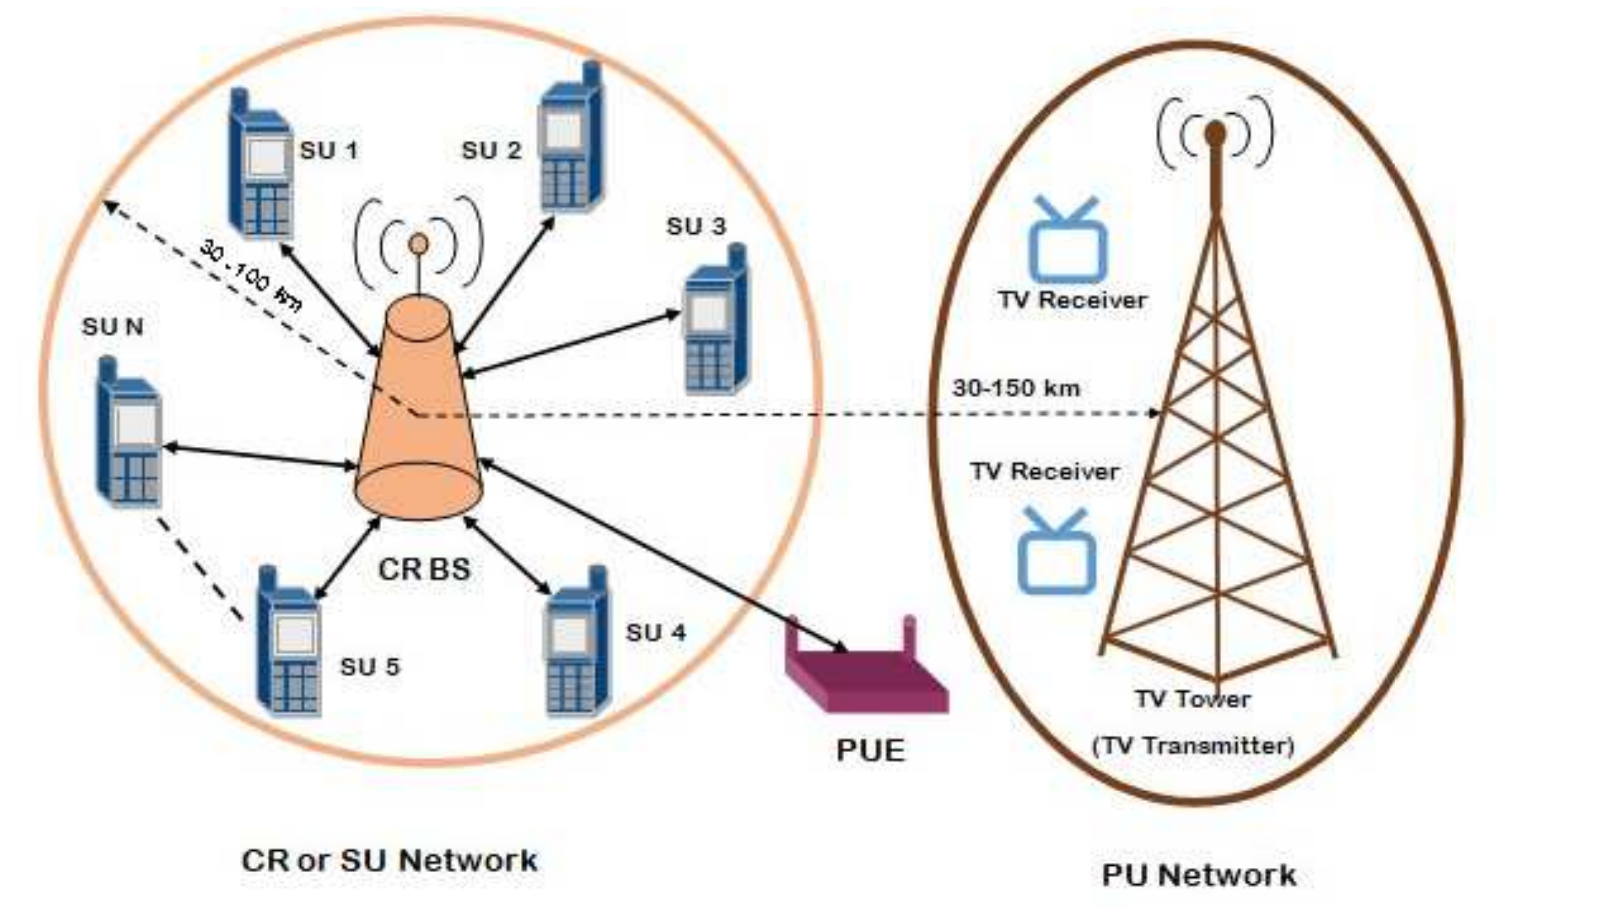
\includegraphics[width=0.9\linewidth]{Figures/chapter1/location-based PUEA detection.png}
    \caption{Location-based PUEA detection \cite{ref20}}
    \label{fig:enter-label}
\end{figure}

\subsection{Signal Characteristic-based Methods}
Several researchers have exploited unique signal characteristics to identify PUEA \cite{ref11,ref6}. For instance, \cite{ref11} utilized cyclostationarity features of signals, while employed cross-layer detection techniques combining PHY and MAC layer information \cite{ref5}. These approaches typically perform well in controlled environments but may struggle when attackers precisely mimic legitimate signal characteristics\cite{ref17}.

\subsection{Machine Learning-based Methods}
Recent years have witnessed growing interest in applying machine learning techniques for PUEA detection  \cite{ref9, ref23}. These approaches train classifiers using features extracted from signal measurements to distinguish between legitimate and malicious transmissions \cite{ref22,ref19}. While promising, many existing machine learning approaches have not been systematically evaluated across varying spatial scenarios and attacker presence levels \cite{ref13}.
